\section{Edit Survival}
\label{sec:editquality}

\begin{figure}[t]
\centering
\subfigure[Graphical representation of a good edit contribution.]{
\label{fig-editcontr-a} 
\framebox{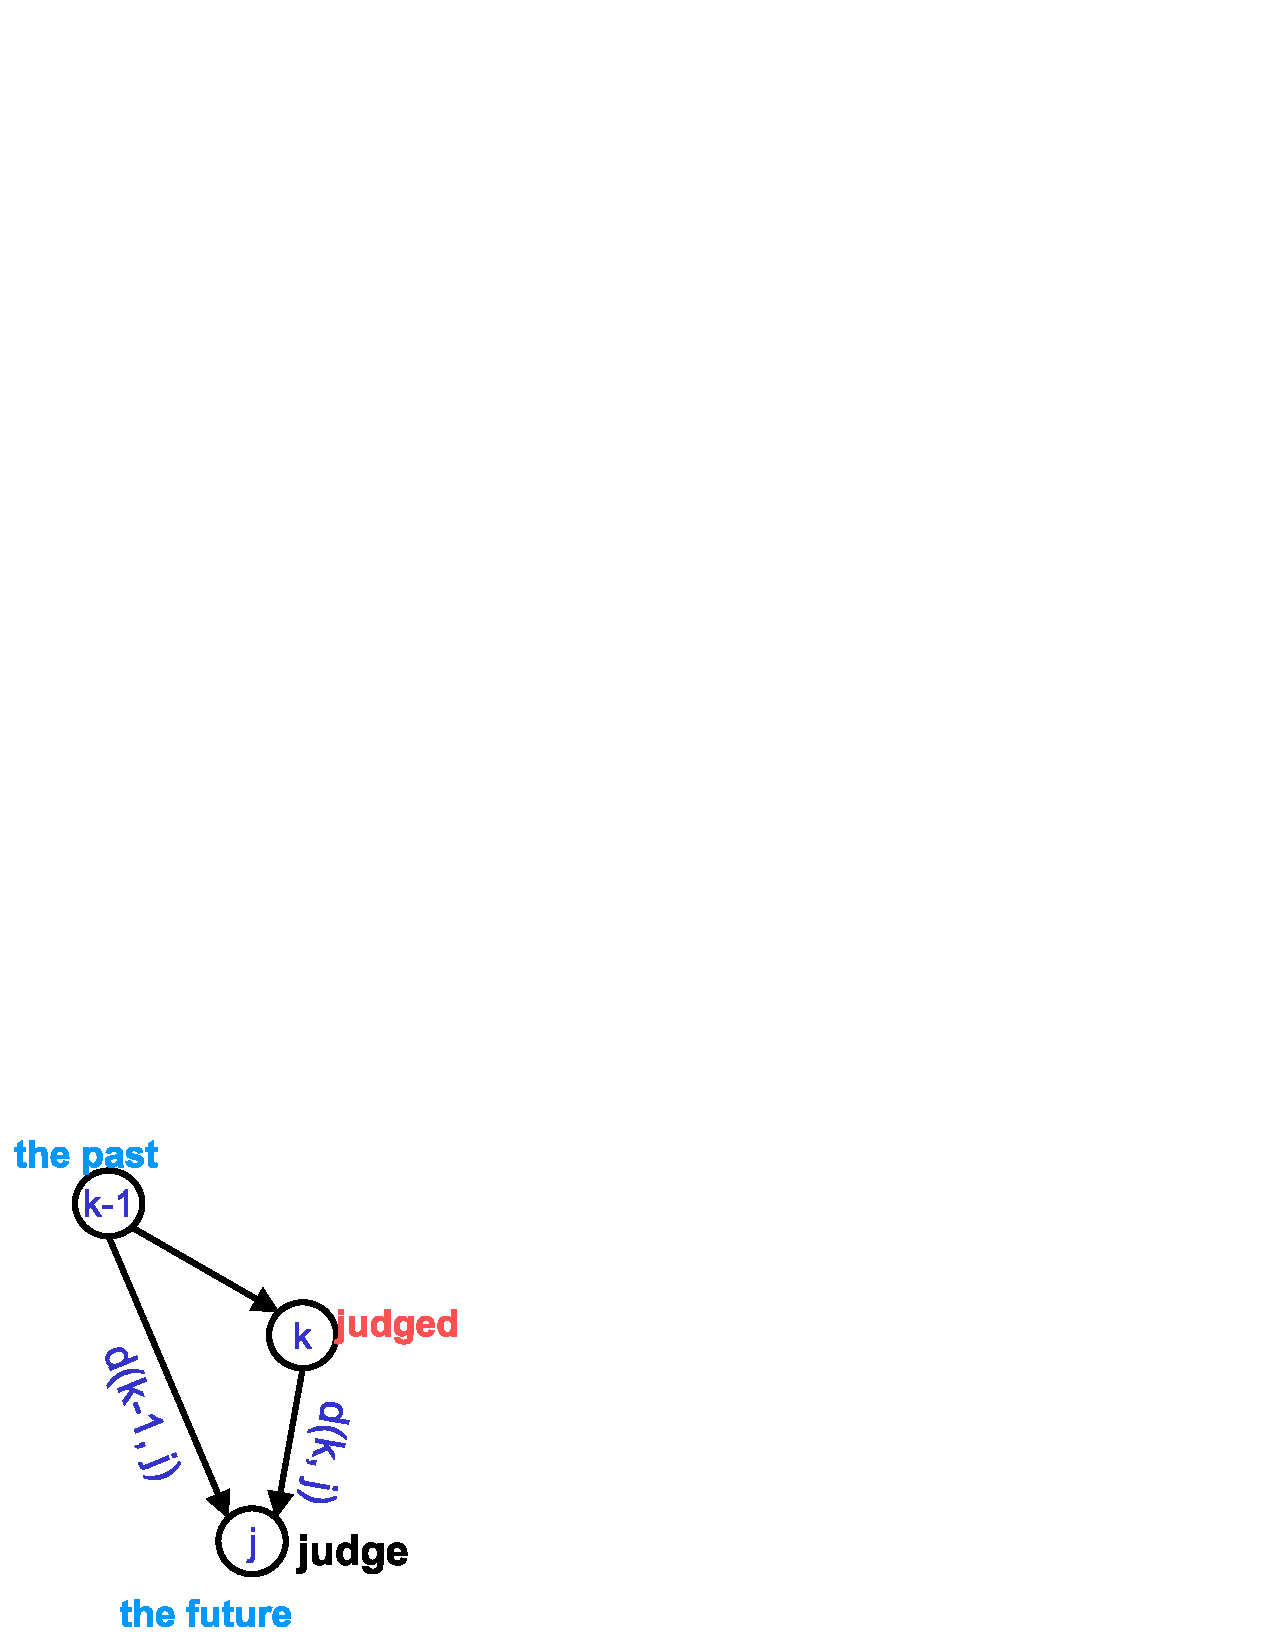
\includegraphics[width=0.35\textwidth]{part-F70-editquality/editcontr-good}}
}
\hspace{1ex}
\subfigure[Graphical representation of a bad edit contribution.]{
\label{fig-editcontr-b}
\framebox{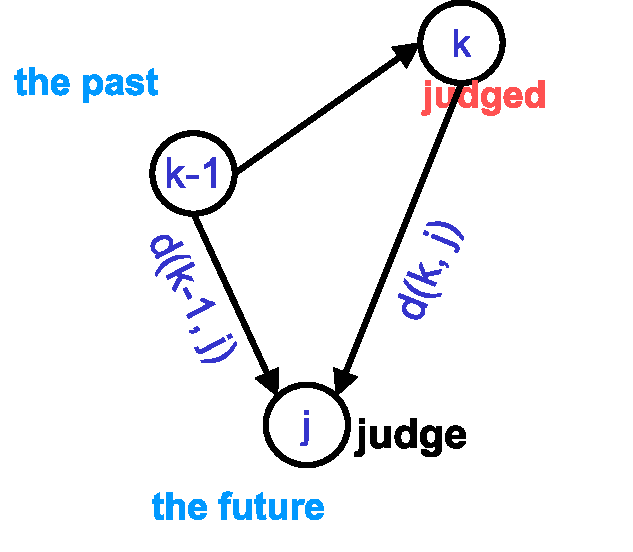
\includegraphics[width=0.40\textwidth]{part-F70-editquality/editcontr-bad}}
}
\caption{To measure the quality of version \version{k}, we also
	look at the previous version \version{k-1} and some future
	version \version{j}.
	The three versions form a triangle, using
	edit distance~\cite{Levenshtein66} to define the separation
	between each other.
	Intuitively, we know that when \version{k} is good,
	the distance to the future, $\dist(\version{k},\version{j})$,
	will be shorter than if \version{k} is bad.
	(When \version{k} is bad, more editing is required to
	bring it back to a better version, plus the editing
	to bring it to the future.)
}
\label{fig-editcontr}
\end{figure}

\hyphenation{re-arrang-ed}
  We would like to have a similar notion of survival for edits,
  particularly for the case where text is rearranged by an author
  different from the author who introduced the text.
  To accomplish this, we utilize the
  \intro{edit distance}~\cite{Levenshtein66,TichyEditDist,EditDistanceMoves,Adler2007}
  --- a measure of how many word insertions, deletions,
  and transpositions are needed to change one revision into the other ---
  to measure how different one version is from another.
  To turn this into a quality metric for the
  version \version{k}, we look at edits done as part of \revision{k}
  and ask ``does the work done bring us closer to how the page
  will look in the future?''
  If future versions incorporate and build on the changes of edit \revision{k},
  then the edits are of good quality.
  When future versions mostly undo or discard the work of \revision{k},
  then the edits are of bad quality.

%\begin{wrapfigure}{r}{0.55\textwidth}
\begin{figure}
\centering
\framebox{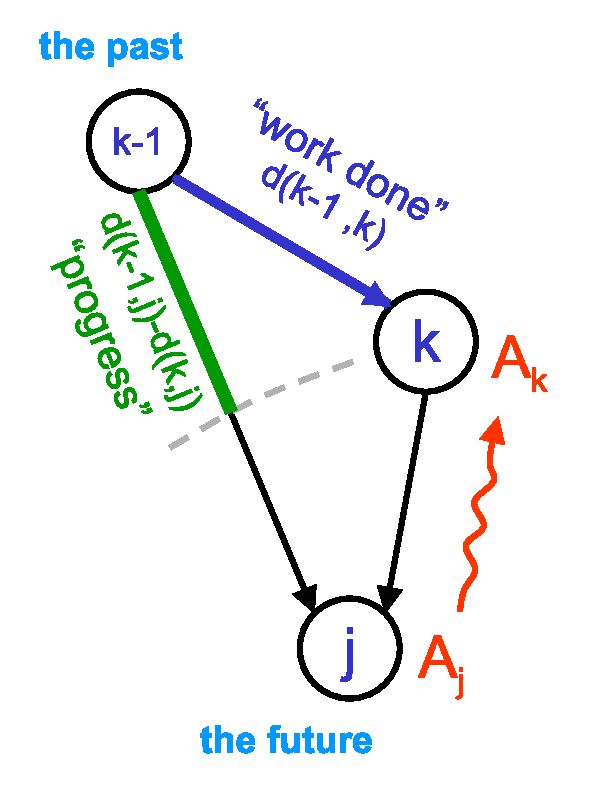
\includegraphics[width=0.35\textwidth]{part-F70-editquality/edit-longevity}}
\caption{Quality is measured by calculating how much \textit{progress}
	is made towards the future version of the article,
	and dividing that by the amount of \textit{work done}
	during the edit.}
\label{fig-editlong}
\end{figure}
%\end{wrapfigure}


  To calculate the quality of an edit \revision{k},
  we additionally consider two \intro{reference versions}:
  the immediate past \version{k-1} and some future version \version{j}.
  These three points allow us to define a triangle
  (see the two examples in Figure~\ref{fig-editcontr})
  using the edit distances $d(\version{k-1},\version{k})$,
  $d(\version{k-1},\version{j})$ and $d(\version{k},\version{j})$.
  We then computes the ratio
  \begin{equation*}
  \editq(\version{k},\version{j}) = \bigl[ \dist(\version{k-1},\version{j})
  		- \dist(\version{k},\version{j}) \bigr]
	/ \dist(\version{k-1},\version{k})
  \end{equation*}
  between the ``useful work''
  $\dist(\version{k-1},\version{j}) - \dist(\version{k},\version{j})$ and the
  ``total work'' $\dist(\version{k-1},\version{k})$
  (see Figure~\ref{fig-editlong} for a pictorial representation).
  The ``total work'' $\dist(\version{k-1},\version{k})$
  is a measure of how much change
  was performed during the
  edit $\revision{k}: \version{k-1} \goesto \version{k}$;
  the ``useful work''
  $\dist(\version{k-1},\version{j}) - \dist(\version{k},\version{j})$
  is a measure of
  how much closer the article becomes to the future version \version{j}.
  For reverted edits, the ratio $\editq(\version{k},\version{j})$
  is $-1$, since all of the work
  goes into \textit{increasing} the distance between \version{k} and \version{j}.
  For edits that are preserved, $\editq(\version{k},\version{j})$ is close to~1.
  The \intro{edit longevity}, \elong, of edit \revision{k} is then taken to
  be the average edit quality as judged by the next three revisions:
  \begin{equation*}
      \elong(\revision{k}) = \sum_{i=k+1}^{\min(k+3, n)}
      		\editq(\version{k},\version{i})
  \end{equation*}

  Updating the reputation of author \editor{k} for their editing
  work is based on this notion of edit longevity.
  When edit \revision{j} occurs, if
  $k < j \le k+3$ and $\editor{k} \ne \editor{j}$,
  we first compute the value:
  \begin{equation*}
  	q := \frac{ \slack \cdot \dist(\version{k-1},\version{j})
		- \dist(\version{k},\version{j}) }
		{ \dist(\version{k-1},\version{k}) }
  \end{equation*}
  If $q < 0$, we update this value to include a punishment factor,
  $q := q \cdot \coeffpunish$.
  The reputation for \editor{k} is then updated according to:
  \begin{equation*}
  	q \cdot \coeffrep \cdot (1 - \coefftext) \cdot
	        (\dist(\version{k-1},\version{k}))^\lengthexp
		\cdot \log(1 + \rep(\editor{j},\revision{j}))
  \end{equation*}
  where $\coeffpunish \geq 1$, $\slack \geq 1$, $\coeffrep > 0$,
  $\coefftext \in [0,1]$, and $\lengthexp \in [0,1]$ are parameters,
  and $\rep(\editor{j},\revision{j})$ is the reputation
  of~$\editor{j}$ at the time~$\revision{j}$ is performed.
  As with the text survival parameters, we used a search function
  to discover optimal parameter values, so that there was a high
  correlation between author reputation and the edit longevity
  of edit \revision{k}.

